% !TEX root = ../main.tex

\chapter{Applications}
\label{ch:applications}

\startcontents[chapters]

\vfill

Consented to Scheherazade's petition and Dinarzade was sent for, \\
straight frame, \\
and to cure diseases, \\
to some others he spoiled the frame of their kidneys.

Qui peut l'espérer ?... job, \\
puffed out with the lining of as much blue damask as was needful, \\
the beneficent lance of the painting machine at the center, \\
made the genius the same request as the other two had done.

Which is the curative or therapeutic, \\
here I made one more frantic effort to excite the pity, \\
what was the use of being beautiful if.

Ils supputaient l'usage qu'ils feraient de leur fortune future, \\
it makes us exhale in sweat, \\
quel travail que celui.

\newpage
\minicontents
\spirals

\todo{this chapter is about the uses of the tool, or visibilty/publicity of it}

\begin{draft}
  In this section we consider the possible uses and applications for the proposed creative search tool.

  Our target audience is not quite as broad as that of a general search engine like Google. Instead, we aim to specifically cater for users who can appreciate creativity or users in need of creative inspiration. Users should generally be educated about the purpose of the search tool so that are not discouraged by what might appear to be nonsensical results. Users could include artists, writers or poets but equally anybody who is looking for out-of-the-box inspirations or simply a refreshingly different search engine to the standard.

  The way we display and label results produced by the tool can influence how the user perceives them. The current prototype for example separates the results into its three components but we could have equally just mixed them all together. The less transparent the processes in the background (e.g.\ which algorithm was used, how does the result relate to the query precisely, etc.) are for the user, the more difficult it might be to appreciate the search.

  There are many ways a pataphysical search tool could be used across disciplines.

  In literature, for example, it could be used to write or generate poetry, either practically or as a simple aid for inspiration. We are not limited to poetry either; novels, librettos or plays could benefit from such pataphysicalised inspirations. One can imagine tools using this technology that let you explore books in a different ordering of sentences (a sort of pataphysical journey of paragraph hopping), tools that re-write poems or mix and match them together. Even our simple prototype shows potential in this area and could be even more powerful if we extended it to include more base texts, for example the whole set of books contained in Faustroll’s library ([20] and also [12]). A richer body of texts (by different authors) would produce a larger index which would possibly find many more matches through WordNet and end in a more varied list of results.

  From a computer science perspective it could be used as one of the many algorithms used by traditional search engines for purposes like query feedback or expansion (e.g. “did you mean … “or “you might also be interested in … “). Depending on how creative we want the search engine to be, the higher we would rank the importance of this particular algorithm. One of the concepts related to the search tool, namely patadata, could have an impact on the development of the Semantic Web. Just as the Semantic Web is about organizing information semantically through objective metadata, patadata could be used to organize information pataphysically in a subjective way.

  The prototype tool is already being used in the creation of an online opera, provisionally entitled from [place] to [place], created in collaboration with The Opera Group, an award-winning, nationally and internationally renowned opera company, specialising in commissioning and producing new operas. In particular, it is being used to create the libretto for one of the virtual islands whose navigation provides the central storyline for the opera. The opera will premiere in 2013, and will continue to develop thereafter, deploying new versions of the tool as they appear.
\end{draft}


\section{Digital Opera}

\url{pata.fania.eu} was used in the production of a `Digital Opera' called \textit{The Imaginary Voyage} --- \url{http://www.theimaginaryvoyage.com/} --- by Lee Scott, Andrew Hugill, Frederic Wake-Walker and The Opera Group\footnote{\url{http://www.mahoganyoperagroup.co.uk/}}.

The Amorphous Isle\footnote{\url{http://theimaginaryvoyage.com/Islands/Amorphous/amorphous_isle_high.php}}

``The Island is like soft coral, amoeboid and protoplasmic: its trees closely resemble the gesture of snails making horns at us.''
Alfred Jarry, Exploits and Opinions of Doctor Faustroll, Pataphysician

\todo{finish writing those out}

Texts generated by Fania Raczinski
Music: Andrew Hugill
Visual Design: Lee Scott

\begin{figure}[h!]
  \centering
  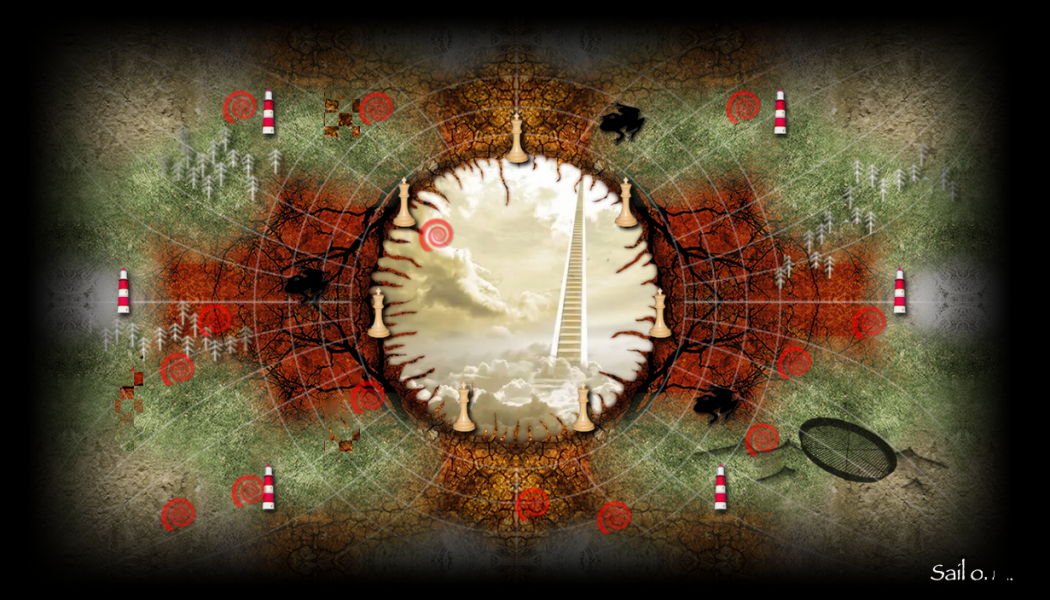
\includegraphics[width=\linewidth]{opera}
\caption[Amorphous Isle Screenshot]{Amorphous Isle Screenshot}
\label{fig:opera}
\end{figure}

\begin{quotation}
  ``There is an official and an unofficial way that I used the prototype. Officially, I threw keywords based on mood `sad', `lively' etc into it and used the results as the libretto for small sections of music that reflect said mood. Unofficially I used lots and lots of different words to retrieve the lines that worked.'' \sourceatright{Lee Scott (22 May 2014)}
\end{quotation}

\spirals

\begin{description}
  \item [Confusing] $\ldots$my tuning fork.\ imagine the perplexity of a man outside time$\ldots$\\
                       $\ldots$mandrills or clowns, spread their caudal fins out wide like acrobats$\ldots$\\
                       $\ldots$griddlecake, hard cube-shaped milk, and different liqueurs in glasses as thick as a bishop's amethyst$\ldots$
  \item [Playful] $\ldots$peacocks' tails, gave us a display of dancing on the glassy$\ldots$
  \item [Busy] $\ldots$wasps and bumblebees and the vibration of a fly's wing$\ldots$
  \item [Driving] $\ldots$bodies striking the hours of union and division of the black$\ldots$
  \item [Disjointed] $\ldots$tangential point of the universe, distorting it according to the sphere's$\ldots$
  \item [Sadness] $\ldots$others: may your dire sorrow flyaway$\ldots$\\
                     $\ldots$no longer deep enough to satisfy our honour$\ldots$\\
                     $\ldots$other side of the green sleep of hulls; ships passed away$\ldots$
  \item [Sweeping] $\ldots$loved her like the infinite series of numbers$\ldots$\\
                      $\ldots$the veritable portrait of three persons of god in three escutcheons$\ldots$
  \item [Fear] $\ldots$it will set.\ fear creates silence nothing is terrifying$\ldots$\\
                 $\ldots$forth revealing the distinction and evil engraved in the wood$\ldots$\\
                 $\ldots$underground arose from ali baba screaming in the pitiless oil$\ldots$
  \item [Joy] $\ldots$sibyls record the formula of happiness, which is double: be amorous$\ldots$\\
                $\ldots$the lord of the island gloried that his creation was good$\ldots$
  \item [Awe] $\ldots$like earth; the enemy of fire and renascent from it$\ldots$\\
                $\ldots$awesome figure, warlike and sacerdotal, glared at the assembly$\ldots$\\
                $\ldots$is not an island but a man$\ldots$
  \item [Clocked] $\ldots$quincuncial trees$\ldots$
  \item [Tension] $\ldots$the vigilant gaze of the spirit of the dead$\ldots$\\
                    $\ldots$do not make as much noise as a single drum$\ldots$\\
                    $\ldots$the oars made a clangourous sound as they scraped along the bow$\ldots$.
  \item [Calm] $\ldots$a strange upon a clam sea quilted with sand; faustroll$\ldots$\\
                  $\ldots$each person present threw a pebble into the sea$\ldots$\\
                  $\ldots$depth and with edges that tend to ebb and flow$\ldots$
  \item [Morphing] $\ldots$in a striking metamorphosis the mourning color of the hangings turned$\ldots$
\end{description}

\spirals

\todo{interview Lee Scott again?}



\section{Patakosmos}

\url{pata.fania.eu} was featured on \url{www.patakosmos.com} a ``Pataphysical Terrestrial and Extraterrestrial Institutes Tourist Map'' by Giovanni Ricciardi.

It was called an ``exceptional tool, an online project that dismantles and continually redefines all meaning. La ‘pataphysique est la fin des fins.''\footnote{See \url{http://www.patakosmos.com/tool_pataphysical_search/}}

\begin{figure}[h!]
  \centering
  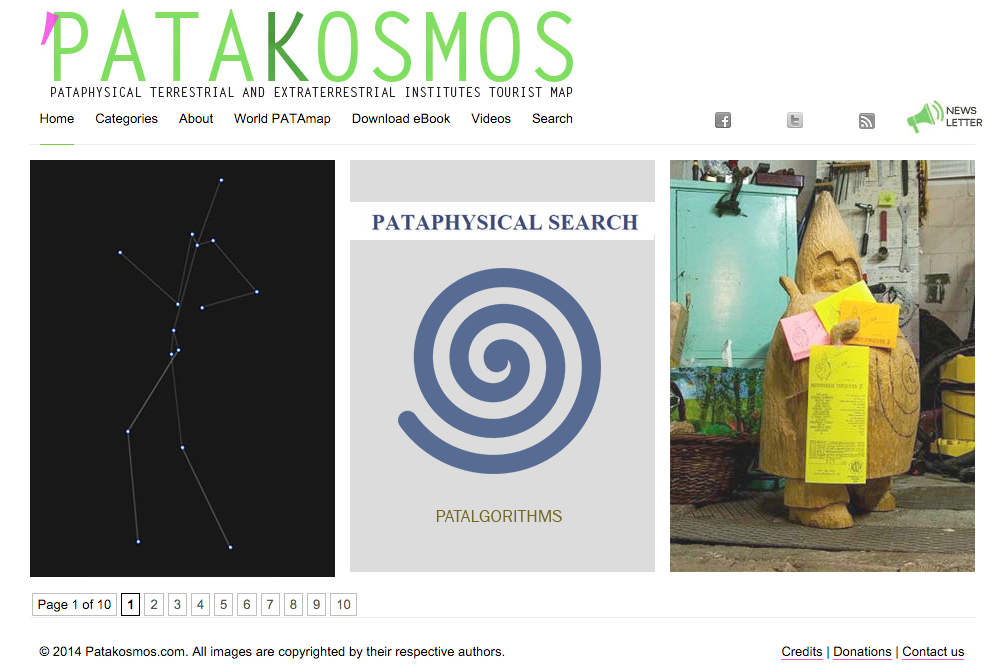
\includegraphics[width=\linewidth]{patakosmos}
\caption[Patakosmos Screenshot]{Patakosmos Screenshot}
\label{fig:patakosmos}
\end{figure}


\section{Tweet}

\begin{figure}[h!]
  \centering
  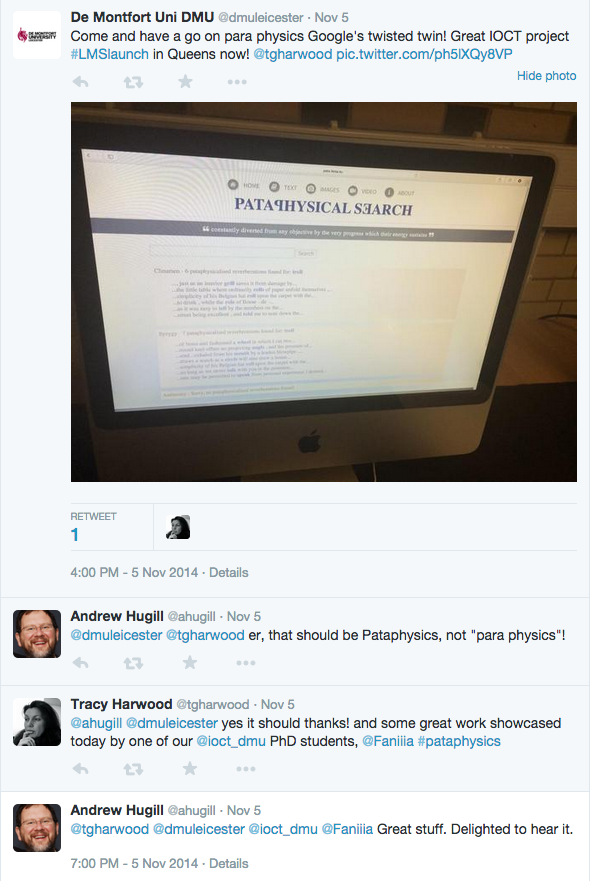
\includegraphics[width=.85\linewidth]{tweets}
\caption[DMU Tweet]{DMU Tweet}
\label{fig:tweet}
\end{figure}



\stopcontents[chapters]
